%%==================================================
%% chapter02.tex for TJU Master Thesis
%% based on CASthesis
%% modified by wei.jianwen@gmail.com
%% Encoding: UTF-8
%%==================================================

\chapter{论文主要内容实例}



\section{图}

\begin{figure*}[!htbp]
	\centering
	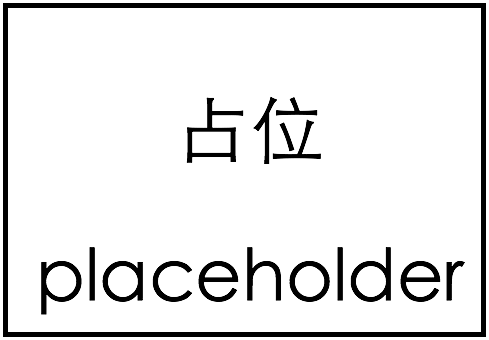
\includegraphics[width=0.5\linewidth]{figure/placeholder}
	\fcaption{中文标题}{英文标题}[目录标题]
	\label{fig:placeholder}
\end{figure*}

\subsection{子图}

\begin{figure*}[!htbp]
	\centering
	\subfigure[]{
			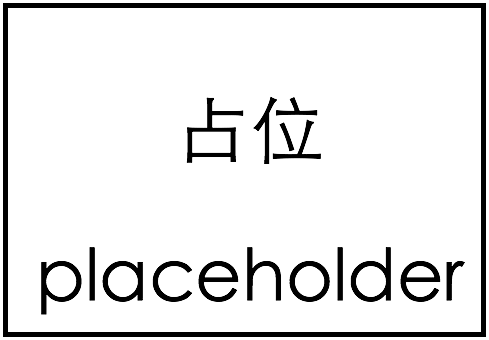
\includegraphics[width=0.45\linewidth]{figure/placeholder}
			\label{fig:subfigure-sub-1}
		}
		\vspace{0.5cm}
	\subfigure[]{
		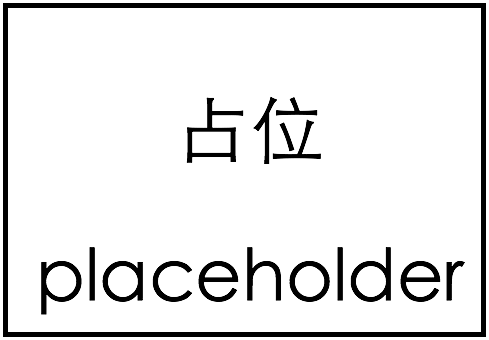
\includegraphics[width=0.45\linewidth]{figure/placeholder}
		\label{fig:subfigure-sub-2}
	}
	\fcaption{中文标题}{英文标题}[目录标题-2]
	\label{fig:subfigure}
\end{figure*}

\newpage
\section{表}

\begin{table}[!htbp]

	\centering
	\tcaption{中文表标题}{英文表标题}[表格表标题]
	\label{tab:table-example}

	
	\begin{tabular*}{0.7\textwidth}{@{\extracolsep\fill}>{\hspace{0.5cm}}ccc<{\hspace{0.5cm}}}
		\toprule
					   &       研究内容        &     研究方法      \\
		\midrule
		研究对象  &       研究内容        &     研究方法      \\
		研究对象  &       研究内容        &     研究方法      \\
	 	研究对象  &       研究内容        &     研究方法      \\
		研究对象  &       研究内容        &     研究方法      \\
		\bottomrule
	\end{tabular*} 
	
\end{table}









